
%(BEGIN_QUESTION)
% Copyright 2006, Tony R. Kuphaldt, released under the Creative Commons Attribution License (v 1.0)
% This means you may do almost anything with this work of mine, so long as you give me proper credit

Her vises en P\&ID (Prosess og instrumenteringsdiagram) for en væskestrøm reguleringssløyfe. Den består av en strømningsmåler (FT) som registrer strømningen i røret og sender et elektronisk signal på for stor strømning det er. En strømingsregulator (FC) mottar signalet og sammenligner dette med et settpunkt, for så å avgjør hvilken vei reguleringsventilen skal bevege seg. En strøm til luft omformer (*(FY) konverterer strømsignalet fra regulatoren til et lufttrykk som styrer posisjonen til reguleringsventilen(FV), som igjen styrer strømningen i røret. 

$$\includegraphics[width=15.5cm]{i00124x01.eps}$$

Retningen på styresignalet for hvert instrument vises her:

\begin{itemize}
\item{} FT: Økende strømning = økende signal
\item{} FC: Økende signal på inngang (PV) = minkende signal på utgang (MV) 
\item{} FY: økende strømsignal på inngang = økende pneumatisk signal på utgangen 
\item{} FV: økende pneumatisk signal = ventilen åpner mer.
\end{itemize}

Forklar hva som  vil skje med alle signalene i denne reguleringssløyfen med regulatoren i "Auto" modus (Klar for å kompensere for variasjoner i strømningen) hvis pumpen plutselig roterer fortere og øsker strømningen. 

Forklar også hva som vil skje med styresignalene i reguleringssløyfen med regulatoren i "manual" modus(styresignalet står fast på det som operatøren har stilt det på) dersom pumpen roterer fortere og forårsaker en økning i strømningen. 


\vskip 20pt \vbox{\hrule \hbox{\strut \vrule{} {\bf Suggestions for Socratic discussion} \vrule} \hrule}

\begin{itemize}
\item{} Explain the practical benefit of having a ``manual'' mode in a process loop controller.  When might we intentionally use manual mode in an operating process condition?
\end{itemize}

\underbar{file i00124}
%(END_QUESTION)





%(BEGIN_ANSWER)

\noindent
{\bf In automatic mode:}

Process flow rate (increase) $\to$ FT output signal (increase milliamps) $\to$ FC output signal (decrease milliamps) $\to$ FY output signal (decrease PSI) $\to$ FV position (moves further closed, pinching off liquid flow).

\vskip 10pt

\noindent
{\bf In manual mode:}

Process flow rate (increase) $\to$ FT output signal (increase milliamps) $\to$ FC output signal (remains steady) $\to$ FY output signal (remains steady) $\to$ FV position (holds position).

\vskip 10pt

The important part of this question is the difference in response between ``automatic'' and ``manual'' controller modes.  In automatic control mode, the controller takes action to bring the process back to setpoint.  In manual control mode, the controller just lets the process drift and takes no action to stop it.

At first, having a ``manual'' mode in a control system seems pointless.  However, giving human operators the ability to manually override the otherwise automatic actions of a control system is important for start-up, shut-down, and handling emergency (unusual) conditions in a process system.  

Manual mode is also a very important diagnostic tool for instrument technicians and operators alike.  Being able to ``turn off the brain'' of an automatic control system and watch process response to manual changes in manipulated variable (final control element) signals gives technical personnel opportunity to test for unusual control valve behavior, process quirks, and other behaviors in a system that can lead to poor automatic control. 


%(END_ANSWER)





%(BEGIN_NOTES)




%INDEX% Control, basics: signal changes in an automatic control loop

%(END_NOTES)


